\documentclass [11pt]{article}
%Needed for fancy maths stuff
\usepackage{amsmath}
%Needed for Wits Style
\usepackage{url}
\usepackage{natbib} % Force natbib.sty to put citation labels in the reference list
\makeatletter
\renewcommand\NAT@biblabel[1]{\def\citeauthoryear##1##2{##1 ##2}[#1]\hfill}
\renewcommand\NAT@bibsetup[1]{%
  \setlength{\itemsep}{\bibsep}\setlength{\parsep}{\z@}}
\def\@lbibitem[#1]#2{%
  \if\relax\@extra@b@citeb\relax\else
    \@ifundefined{br@#2\@extra@b@citeb}{}{%
     \@namedef{br@#2}{\@nameuse{br@#2\@extra@b@citeb}}}\fi
   \@ifundefined{b@#2\@extra@b@citeb}{\def\NAT@num{}}{\NAT@parse{#2}}%
   \item[\hfil\hyper@natanchorstart{#2\@extra@b@citeb}\@biblabel{#1}%
    \hyper@natanchorend]%
    \NAT@ifcmd#1(@)(@)\@nil{#2}}
\makeatother


\bibpunct{[}{]}{;}{a}{}{}
%For figures
\usepackage{graphicx}
\usepackage{float}

\title{Building Bayesian Influence Ontologies\\Literature Review}
\author{Tamlin Love\\1438243}
\date{\today}

\usepackage[margin=1in]{geometry} %Margin size

\begin{document}
\maketitle
\section{Introduction}

\section{Similarity Metrics}\label{SimilarityMetrics}
\section{Bayesian Networks}\label{BayesianNetworks}
When considering a joint probability distribution across $n$ random variables, classical probability states that the number of parameters needed to represent the distribution grows exponentially in $n$ \citep{koller09}. Even in the simple case of binary variables, we would still need $2^n -1$ parameters to describe the distribution. This is clearly unfeasible for practical applications, in which the number of random variables can grow very large. 
\\
Bayesian networks, originally developed by \citet{pearl88}, present a way of reducing the number of parameters needed to represent a joint distribution. A Bayesian network is a directed acyclic graph (DAG) whose nodes represent random variables and whose edges represent influence of one variable on another. This structure can also be thought of as a representation of the conditional independencies between the random variables \citep{koller09}. Indeed, it is through the exploitation of these independency assumptions that a Bayesian network can more compactly represent a joint distribution.
\begin{figure}[H]\label{fig:sprinkler}
\centering
\caption{A famous example of a Bayesian network, showing how a complete representation of any random variable $X$ requires considering only those variables who are parents of $X$ in the graphical representation \citep{norvig94}.}
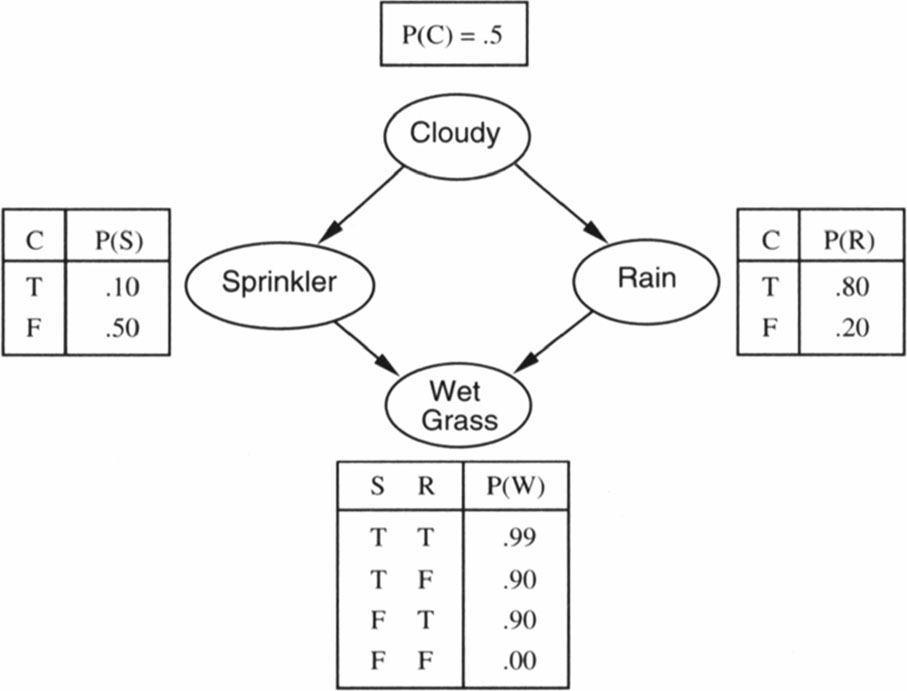
\includegraphics[width=8cm]{sprinkler.jpg}
\end{figure}
An important notion in Bayesian networks is that of d-separation, first presented by \citet{pearl86}, which is used to find the set $\mathcal{I}(\mathcal{G})$ of conditional independencies in the graph $\mathcal{G}$. $\mathcal{I}(\mathcal{G})$ is used as the basis for an equivalence relation, I-equivalence, for which any two I-equivalent graphs represent the same independency assumptions \citep{verma91}. An important developement by \citet{pearl86} is that any I-equivalence class can be represented as a partially directed acyclic graph (PDAG) in which undirected edges represent edges that can be oriented any way and still result in a graph belonging to the same class.
\section{Structure Learning}\label{StructureLearning}
The manual construction of networks is generally unfeasible for a large number of variables \citep{koller09}. Fortunately, strategies exist to learn model structures from data $\mathcal{D}$.
\subsection{Constraint-Based Structure Learning}
One approach to the construction of model structures is the constraint-based approach, in which dependencies between variables are first queried and then, based on these dependencies, a PDAG is constructed \citep{koller09}. This strategy can be traced back to \citet{verma91}. 
\\
However, this approach is generally not preferred, as failure in the individual independence queries can lead to the construction of a network which poorly matches the data \citep{koller09}.
\subsection{Score-Based Structure Learning}
A more popular approach to the problem is score-based structure learning, in which entire networks are constructed and then evaluated and modified based on some scoring metric \citep{koller09}.
\section{Bayesian Similarity}\label{BayesianSimilarity}
\bibliographystyle{named-wits}
\bibliography{annot}
\end{document}